\section{Boundary Treatment}
\label{sec:24boundary}

\minitoc{79mm}{5}

\noindent
One issue of regular sparse grids $\regsgset{n}{d}$
is that the number of grid points still grows very fast
with the level $n$ and the dimensionality $d$ \cite{Pflueger10Spatially}.
This is mainly because the finest mesh size $\ms{n}$ on the
boundary of the domain $\clint{\*0, \*1}$ is finer than
the finest mesh size $\ms{n-d+1}$ that can be found in the interior.
If we define $\interiorregsgset{n}{d}$ as the set of
interior grid points in $\regsgset{n}{d}$,%
\footnote{%
  Note that in the literature (e.g., \cite{Pflueger10Spatially}),
  the regular sparse grid space of level $n$ without boundary points is often
  defined via $\normone{\*l} \le n + d - 1$ to ensure that the finest mesh size
  is given by $\ms{n}$.
  In our notation, this corresponds to $\interiorregsgset{n+d-1}{d}$.%
}
i.e.,
\begin{equation}
  \interiorregsgset{n}{d}
  \ceq \regsgset{n}{d} \cap \opint{\*0, \*1}
  = \{\gp{\*l,\*i} \in \regsgset{n}{d} \mid \*l \ge \*1\},
\end{equation}
then the following relation about the number of grid points
of $\regsgset{n}{d}$ can be shown:

\begin{lemma}[number of regular sparse grid points]
  \label{lemma:numberOfGridPointsBoundary}
  \setlength{\abovedisplayskip}{0pt}%
  \begin{equation}
    \setsize{\regsgset{n}{d}}
    = \sum_{q=0}^d 2^q \binom{d}{q} \setsize{\interiorregsgset{n}{d-q}}
  \end{equation}
\end{lemma}
\begin{proof}
  See \cite{Bungartz04Sparse}.
\end{proof}
Here, we define zero-dimensional grids to contain exactly one grid point
such that $\setsize{\interiorregsgset{n}{0}} = 1$.
The number of interior grid points can be calculated as follows:
\begin{lemma}[number of interior regular sparse grid points]
  \label{lemma:numberOfGridPointsInterior}
  \setlength{\abovedisplayskip}{0pt}%
  \begin{equation}
    \setsize{\interiorregsgset{n}{d}}
    = \sum_{q=0}^{n-d} 2^q \binom{d-1+q}{d-1}
  \end{equation}
\end{lemma}
\begin{proof}
  See \cite{Bungartz04Sparse}.
\end{proof}

Intuitively, \cref{lemma:numberOfGridPointsBoundary} splits the sparse grid
$\regsgset{n}{d}$ into lower-dimensional sparse grids
$\interiorregsgset{n}{d-q}$ of the same level, but without boundary points.
The factor $2^q \binom{d}{q}$ is the number of $(d-q)$-dimensional faces
of the $d$-dimensional unit hyper-cube.
In the three-dimensional example of \cref{fig:sgDecompose},
the unit cube $\clint{0, 1}^3$ decomposes into
\begin{itemize}
  \item
  $2^0 \binom{3}{0} = 1$ interior cube $\opint{0, 1}^3$,
  
  \item
  $2^1 \binom{3}{1} = 6$ sides (two-dimensional faces)
  like $\opint{0, 1}^2 \times \{0\}$,
  
  \item
  $2^2 \binom{3}{2} = 12$ edges (one-dimensional faces)
  like $\opint{0, 1} \times \{(0, 0)\}$, and
  
  \item
  $2^3 \binom{3}{3} = 8$ corners (zero-dimensional faces)
  like $(0, 0, 0)$.
\end{itemize}
On each of these $(d-q)$-dimensional faces,
the sparse grid $\regsgset{n}{d}$ contains
the interior of a sparse grid of level $n$ and dimensionality $d - q$,
the size of which grows like $\landauO{2^n n^{d-q-1}}$.
As the number of boundary faces increases exponentially
with the dimensionality $d$,
the size of $\regsgset{n}{d}$ quickly exhausts the available
computational memory.
To deal with this issue, there are mainly two solutions,
which are described below.

\begin{figure}
  \raisebox{-0.5\height}{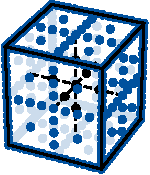
\includegraphics{sgDecompose_1}}%
  \raisebox{-0.5\height-0.5mm}{$\;\;=\;\;$}%
  \raisebox{-0.5\height}{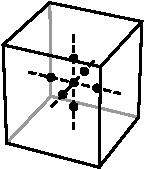
\includegraphics{sgDecompose_2}}%
  \raisebox{-0.5\height}{$\;\;\dotcup\;\;$}%
  \raisebox{-0.5\height}{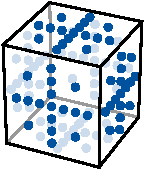
\includegraphics{sgDecompose_3}}%
  \raisebox{-0.5\height}{$\;\;\dotcup\;\;$}%
  \raisebox{-0.5\height}{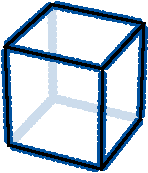
\includegraphics{sgDecompose_4}}%
  \raisebox{-0.5\height}{$\;\;\dotcup\;\;$}%
  \raisebox{-0.5\height}{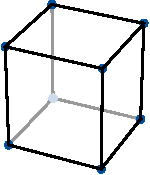
\includegraphics{sgDecompose_5}}%
  \caption[%
    Decomposition of a sparse grid into lower-dimensional sparse sub-grids%
  ]{%
    Decomposition of the three-dimensional sparse grid $\regsgset{n}{d}$
    ($n = 4$, $d = 3$) into lower-dimensional sparse sub-grids.
    The main axes (axis-parallel lines through $0.5 \cdot \*1$, \emph{dashed})
    serve as a visual aid.%
  }%
  \label{fig:sgDecompose}%
\end{figure}



\subsection{Sparse Grids with Coarser Boundaries}
\label{sec:241coarseBoundary}

\paragraph{Inserting boundary points at higher levels}

The first solution is to insert the boundary level functions and grid points
at a higher level than at level zero.
A popular choice is the insertion at level one, which corresponds to
\begin{equation}
  \label{eq:sparseGridB1}
  \coarseregsgset{n}{d}{1}
  \ceq \bigdotcup_{\*l \in \coarselevelset{n}{d}{1}}
  \{\gp{\*l,\*i} \mid \*i \in \hiset{\*l}\},\quad
  \coarselevelset{n}{d}{1}
  \ceq \{\*l \in \natz^d \mid \normone{\vecmax(\*l, \*1)} \le n\},
\end{equation}
where $\vec{\max}$ is to be read coordinate-wise as usual.
This choice is equivalent to treating zero-level components as level one
in the subspace selection.
This ensures that the finest mesh sizes in the interior of
$\clint{\*0, \*1}$ and on its boundary coincide to be $\ms{n-d+1}$,
which reduces the number of grid points on the boundary significantly.

Another solution that can be found in the literature of sparse grids with
hat functions \cite{Baar15Gradient}
is to start with the ``constant one'' function on level zero with
corresponding grid point $0.5$,
then employ the two boundary functions and points on level one,
and finally proceed as usual for the higher levels $\ge 2$.
Apart from a constant shift of the resulting sparse grid levels,
this is equivalent to inserting the boundary functions and points at level two.
This solution leads to even less grid points than the previous approach,
as now the mesh size is finer in the interior of the domain than on the
boundary.
However, for very high dimensionalities this might still lead to
computationally infeasible sparse grids.

\paragraph{Regular sparse grids with coarse boundary}

\usenotation{zzzzsb}
We generalize these two solutions to the definition of a
sparse grid $\coarseregsgset{n}{d}{b}$ that is equivalent to inserting
the boundary functions and points at an arbitrary level $b \in \nat$:
\begin{definition}[regular sparse grid with coarse boundary]
  \label{def:coarseBoundary}
  The regular sparse grid of level $n \in \nat$,
  dimensionality $d \le n$, and boundary parameter $b \in \nat$ is defined as
  \begin{subequations}
    \begin{align}
      \label{eq:coarseBoundary1}
      \coarseregsgset{n}{d}{b}
      &\ceq \bigdotcup_{\*l \in \coarselevelset{n}{d}{b}}
      \{\gp{\*l,\*i} \mid \*i \in \hiset{\*l}\},\\
      \label{eq:coarseBoundary2}
      \begin{split}
        \coarselevelset{n}{d}{b}
        &\ceq \{\*l \in \nat^d \mid \normone{\*l} \le n\}\\
        &\qquad {} \dotcup \paren*{
          \{\*l \in \natz^d \setminus \nat^d \mid
          \normone{\vecmax(\*l, \*1)} \le n-b+1\} \cup \{\*0\}
        }.
      \end{split}
    \end{align}
  \end{subequations}
  For convenience, we define
  $\coarseregsgset{n}{d}{0} \ceq \regsgset{n}{d}$.
\end{definition}
The definition is motivated by partitioning the levels $\*l \in \natz^d$
into interior levels ($\*l \in \nat^d$)
and boundary levels ($\*l \in \natz^d \setminus \nat^d$).
By including the levels of the interior grid $\interiorregsgset{n}{d}$,
the mesh size in the interior is the same as before ($\ms{n-d+1}$).
Like in \eqref{eq:sparseGridB1}, we treat boundary levels as level one,
but we subtract $b - 1$ from the upper bound to ensure the correct
mesh size $\ms{n-d-b+2}$ on the boundary.
We append $\*0$ to the level set to ensure that at least the $2^d$ corner
points are included in the resulting sparse grid.
Note that this definition is consistent with \eqref{eq:sparseGridB1} as
$\coarselevelset{n}{d}{b}
= \{\*l \in \natz^d \mid \normone{\vecmax(\*l, \*1)} \le n\}$
for $b = 1$.
Examples of~$\coarseregsgset{n}{d}{b}$ are shown
in \cref{fig:coarseBoundary}.
The flip book animation in the bottom right corner of the
odd-numbered pages of this thesis
visualizes $\coarseregsgset{n}{d}{b}$ for $n = 4$, $d = 3$, and $b = 1$.

The number of grid points of $\coarseregsgset{n}{d}{b}$
can be calculated as follows:
\begin{restatable}[number of regular sparse grid points with coarse boundary]{%
  proposition%
}{%
  propGridSizeCoarseBoundary%
}
  \label{prop:gridSizeCoarseBoundary}
  \setlength{\abovedisplayskip}{0pt}%
  \begin{equation}
    \setsize{\coarseregsgset{n}{d}{b}}
    = \setsize{\interiorregsgset{n}{d}} +
    \sum_{q=1}^d 2^q \binom{d}{q}
    \setsize{\interiorregsgset{n-q-b+1}{d-q}},\quad
    b \in \nat
  \end{equation}
\end{restatable}
\begin{proof}
  See \cref{sec:a111proofGridSizeCoarseBoundary}.
\end{proof}
As can be seen in \cref{tbl:coarseBoundary3D} for three dimensions and
in \cref{tbl:coarseBoundary10D} for ten dimensions,
the number of grid points decreases drastically for increasing values
of $b$, especially when compared with
$\regsgset{n}{d} = \coarseregsgset{n}{d}{0}$.

\begin{table}
  \newcommand*{\myheader}{$\setsize{\interiorregsgset{n}{d}}$}%
  \setnumberoftableheaderrows{2}%
  \begin{tabular}{%
    >{\kern\tabcolsep}=l<{\kern7mm}+r<{\kern7mm}+r+r+r+r+r+r<{\kern\tabcolsep}%
  }
    \toprulec
    \headerrow
    &&\multicolumn{6}{c}{%
      $\setsize{\coarseregsgset{n}{d}{b}}/\setsize{\interiorregsgset{n}{d}}$%
    }\\
    \headerrow
    &          \myheader&     $b = 0$&    $b = 1$&    $b = 2$&    $b = 3$&    $b = 4$&    $b = 5$\\
    \midrulec
    $n = 3$&     \num{1}& \num{123.0}& \num{27.0}& \num{9.00}& \num{9.00}& \num{9.00}& \num{9.00}\\
    $n = 4$&     \num{7}&  \num{42.4}& \num{11.6}& \num{4.71}& \num{2.14}& \num{2.14}& \num{2.14}\\
    $n = 5$&    \num{31}&  \num{22.7}& \num{7.3}&  \num{3.39}& \num{1.84}& \num{1.26}& \num{1.26}\\
    $n = 6$&   \num{111}&  \num{14.9}& \num{5.3}&  \num{2.75}& \num{1.67}& \num{1.23}& \num{1.07}\\
    $n = 7$&   \num{351}&  \num{10.9}& \num{4.3}&  \num{2.37}& \num{1.55}& \num{1.21}& \num{1.07}\\
    $n = 8$&  \num{1023}&   \num{8.5}& \num{3.6}&  \num{2.13}& \num{1.47}& \num{1.19}& \num{1.07}\\
    $n = 9$&  \num{2815}&   \num{7.0}& \num{3.2}&  \num{1.96}& \num{1.41}& \num{1.17}& \num{1.07}\\
    $n = 10$& \num{7423}&   \num{6.0}& \num{2.9}&  \num{1.83}& \num{1.36}& \num{1.16}& \num{1.06}\\
    \bottomrulec
  \end{tabular}
  \caption[%
    Comparison of regular sparse grid sizes with coarse boundary
    ($d = 3$)%
  ]{%
    For $d = 3$:
    Grid size of the interior grid
    \vspace{-0.33em}%
    $\interiorregsgset{n}{d}$ \emph{(second column)}
    and ratios
    $\setsize{\coarseregsgset{n}{d}{b}}/\setsize{\interiorregsgset{n}{d}}$
    \emph{(beginning with the third column)} of the sizes of
    the grid $\coarseregsgset{n}{d}{b}$ with boundary points
    to the size of the interior grid of the same level.
    The table starts with the first level $n = 3$ for which
    the interior grid $\interiorregsgset{n}{d}$ is not empty.%
  }%
  \label{tbl:coarseBoundary3D}%
\end{table}

\begin{table}
  \newcommand*{\myheader}{$\setsize{\interiorregsgset{n}{d}}$}%
  \setnumberoftableheaderrows{2}%
  \begin{tabular}{%
    >{\kern\tabcolsep}=l<{\kern7mm}+r<{\kern7mm}+r+r+r+r+r+r<{\kern\tabcolsep}%
  }
    \toprulec
    \headerrow
    &&\multicolumn{6}{c}{%
      $\setsize{\coarseregsgset{n}{d}{b}}/\setsize{\interiorregsgset{n}{d}}$%
    }\\
    \headerrow
    &             \myheader&     $b = 0$&     $b = 1$&    $b = 2$&      $b = 3$&      $b = 4$&      $b = 5$\\
    \midrulec
    $n = 10$&       \num{1}& \num{3.3e8}& \num{59049}& \num{1025}& \num{1025.0}& \num{1025.0}& \num{1025.0}\\
    $n = 11$&      \num{21}& \num{4.3e7}& \num{21558}& \num{2813}&   \num{49.8}&   \num{49.8}&   \num{49.8}\\
    $n = 12$&     \num{241}& \num{1.0e7}& \num{10046}& \num{1879}&  \num{246.0}&    \num{5.2}&    \num{5.2}\\
    $n = 13$&    \num{2001}& \num{3.4e6}&  \num{5407}& \num{1211}&  \num{227.2}&   \num{30.5}&    \num{1.5}\\
    $n = 14$&   \num{13441}& \num{1.3e6}&  \num{3213}&  \num{806}&  \num{181.1}&   \num{34.7}&    \num{5.4}\\
    $n = 15$&   \num{77505}& \num{6.2e5}&  \num{2054}&  \num{558}&  \num{140.6}&   \num{32.2}&    \num{6.8}\\
    $n = 16$&  \num{397825}& \num{3.1e5}&  \num{1390}&  \num{401}&  \num{109.5}&   \num{28.2}&    \num{7.1}\\
    $n = 17$& \num{1862145}& \num{1.7e5}&   \num{984}&  \num{298}&   \num{86.5}&   \num{24.2}&    \num{6.8}\\
    \bottomrulec
  \end{tabular}
  \caption[%
    Comparison of regular sparse grid sizes with coarse boundary
    ($d = 10$)%
  ]{%
    For $d = 10$:
    Grid size of the interior grid
    \vspace{-0.33em}%
    $\interiorregsgset{n}{d}$ \emph{(second column)}
    and ratios
    $\setsize{\coarseregsgset{n}{d}{b}}/\setsize{\interiorregsgset{n}{d}}$
    \emph{(beginning with the third column)} of the sizes of
    the grid $\coarseregsgset{n}{d}{b}$ with boundary points
    to the size of the interior grid of the same level.
    The table starts with the first level $n = 10$ for which
    the interior grid $\interiorregsgset{n}{d}$ is not empty.%
  }%
  \label{tbl:coarseBoundary10D}%
\end{table}

\Cref{alg:coarseBoundary} shows how to generate the necessary set of
hierarchical levels.
Its correctness can be formally proven with the following invariant:
\begin{restatable}[invariant of SG generation with coarse boundary]{%
  proposition%
}{%
  propInvariantCoarseBoundary%
}
  \label{prop:invariantCoarseBoundary}
  After iteration $t$ of \cref{alg:coarseBoundary}
  ($t = 1, \dotsc, d$), it holds
  \begin{equation}
    \label{eq:coarseInvariant}
    \begin{split}
      \levelset^{(t)}
      &= \{\*l \in \nat^t \mid \normone{\*l} \le n - d + t\}\\
      &\hphantom{{}={}} {} \dotcup \paren*{
        \{\*l \in \natz^t \setminus \nat^t \mid
        \normone{\vecmax(\*l, \*1)} \le n-d+t-b+1\} \cup \{\*0\}
      }.
    \end{split}
  \end{equation}
\end{restatable}
\begin{proof}
  See \cref{sec:a112proofInvariantCoarseBoundary}.
\end{proof}
\begin{shortcorollary}[correctness of SG generation with coarse boundary]
  \label{cor:algCoarseBoundaryCorrectness}
  \Cref{alg:coarseBoundary} is correct.
\end{shortcorollary}
\begin{proof}
  Follows immediately from \cref{prop:invariantCoarseBoundary}
  by setting $t = d$,
  as then \eqref{eq:coarseInvariant} becomes
  \eqref{eq:coarseBoundary2} from \thmref{def:coarseBoundary}.
\end{proof}

\begin{algorithm}
  \begin{algorithmic}[1]
    \Function{$\coarselevelset{n}{d}{b} = \texttt{computeSGCoarseBoundary}$}{%
      $n$, $d$, $b$%
    }
      \State{$\levelset^{(1)} \gets \{0, 1, \dotsc, n - d + 1\}$}
      \Comment{one-dimensional grid}%
      \label{line:algCoarseBoundary6}
      \For{$t = 2, \dotsc, d$}
        \State{$\levelset^{(t)} \gets \emptyset$}
        \Comment{$t$-dimensional grid}%
        \For{$\*l \in \levelset^{(t-1)}$}
          \If{%
            $\normone{\vecmax(\*l, \*1)} \le n - d + t - b$ or
            $\*l = \*0$%
          }%
          \label{line:algCoarseBoundary1}
            \State{$\levelset^{(t)} \gets \levelset^{(t)} \cup \{(\*l, 0)\}$}
            \Comment{%
              add corners (with $(\*l, 0) \ceq (l_1, \dotsc, l_{t-1}, 0)$)%
            }%
            \label{line:algCoarseBoundary5}
          \EndIf{}
          \If{$\*l \in \nat^{t-1}$}
            \State{$l^\ast \gets n - d + t - \normone{\*l}$}%
            \Comment{add interior points}%
            \label{line:algCoarseBoundary2}
          \Else{}
            \State{%
              $l^\ast \gets n - d + t - b + 1 -
              \normone{\vecmax(\*l, \*1)}$%
            }%
            \Comment{add boundary points}%
            \label{line:algCoarseBoundary3}
          \EndIf{}
          \State{%
            $\levelset^{(t)} \gets \levelset^{(t)} \cup
            \{(\*l, l_t) \mid l_t = 1, \dotsc, l^\ast\}$%
          }
          \Comment{%
            with $(\*l, l_t) \ceq (l_1, \dotsc, l_{t-1}, l_t)$%
          }%
          \label{line:algCoarseBoundary4}
        \EndFor{}
      \EndFor{}
      \State{$\coarselevelset{n}{d}{b} \gets \levelset^{(d)}$}
    \EndFunction{}
  \end{algorithmic}
  \caption[%
    Generation of regular sparse grids with coarse boundary%
  ]{%
    Generation of the sparse grid $\coarseregsgset{n}{d}{b}$
    with coarse boundary.
    Inputs are the level $n \in \nat$, the dimensionality $d \le n$, and
    the boundary parameter $b \in \nat$.
    Output is the level set $\coarselevelset{n}{d}{b}$
    that corresponds to $\coarseregsgset{n}{d}{b}$.%
  }%
  \label{alg:coarseBoundary}%
\end{algorithm}

\begin{figure}
  \subcaptionbox{%
    $d = 2$, $b = 0$%
  }[35mm]{%
    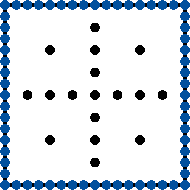
\includegraphics{coarseBoundary_1}%
  }%
  \hfill%
  \subcaptionbox{%
    $d = 2$, $b = 1$%
  }[35mm]{%
    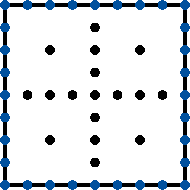
\includegraphics{coarseBoundary_2}%
  }%
  \hfill%
  \subcaptionbox{%
    $d = 2$, $b = 2$%
  }[35mm]{%
    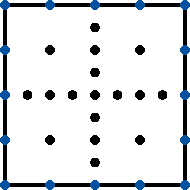
\includegraphics{coarseBoundary_3}%
  }%
  \hfill%
  \subcaptionbox{%
    $d = 2$, $b = 3$%
  }[35mm]{%
    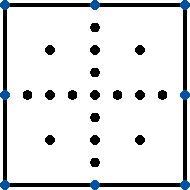
\includegraphics{coarseBoundary_4}%
  }\\[2mm]%
  \subcaptionbox{%
    $d = 3$, $b = 0$%
  }[35mm]{%
    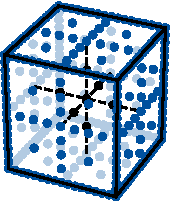
\includegraphics{coarseBoundary_5}%
  }%
  \hfill%
  \subcaptionbox{%
    $d = 3$, $b = 1$%
  }[35mm]{%
    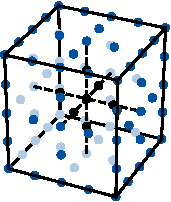
\includegraphics{coarseBoundary_6}%
  }%
  \hfill%
  \subcaptionbox{%
    $d = 3$, $b = 2$%
  }[35mm]{%
    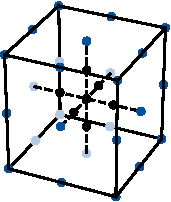
\includegraphics{coarseBoundary_7}%
  }%
  \hfill%
  \subcaptionbox{%
    $d = 3$, $b = 3$%
  }[35mm]{%
    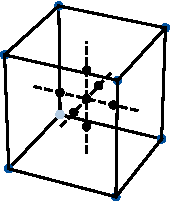
\includegraphics{coarseBoundary_8}%
  }%
  \caption[%
    Comparison of regular sparse grids with coarse boundary%
  ]{%
    Sparse grids $\coarseregsgset{n}{d}{b}$ of level $n = 4$
    in two and three dimensions for different values of the
    boundary parameter $b$.
    For constant $d$ and $n$,
    the points in the interior of $\clint{\*0, \*1}$
    (black) are the same,
    while the points on the boundary of $\clint{\*0, \*1}$
    \emph{\textcolor{mittelblau}{(blue)}} become coarser
    for increasing values of $b$.
    The main axes (axis-parallel lines through $0.5 \cdot \*1$, \emph{dashed})
    serve as a visual aid.%
  }%
  \label{fig:coarseBoundary}%
\end{figure}

\paragraph{Hierarchization and other algorithms}

An important implication of the regular sparse grids
$\coarseregsgset{n}{d}{b}$ as defined in \cref{def:coarseBoundary}
is that, in general,
the unidirectional principle cannot be directly applied anymore.
For example, this is relevant when calculating hierarchical surpluses
for the hat function basis.
As we mostly deal with B-splines, for which the unidirectional
principle cannot be applied even on regular sparse grids,
this issue is not important in the scope of this thesis.

However, it is possible to calculate the hierarchical surpluses
of hat functions on $\coarseregsgset{n}{d}{b}$ in a three-step algorithm.
First, we compute the surpluses of the boundary grid
$\coarseregsgset{n}{d}{b} \setminus \interiorregsgset{n}{d}$.
Second, we subtract the values of the resulting ``boundary interpolant'' at
the inner grid points
$\interiorregsgset{n}{d}$.
Third, we calculate the surpluses of the inner grid points
as usual with the unidirectional principle.
As the corresponding ``inner interpolant'' vanishes
on the boundary, this does not influence the interpolated values in the
first step.



\subsection{Sparse Grids Without Boundary Points and Modified Bases}
\label{sec:242modified}

\paragraph{Omitting boundary points}

The second solution to reduce the number of grid points on the boundary
is to omit the boundary points and the basis functions altogether.
For the hat function basis $\bspl{\*l,\*i}{1}$,
this is a feasible option if the objective
function $\objfun\colon \clint{\*0, \*1} \to \real$
satisfies homogeneous boundary conditions
$\restrictfcn{\objfun}{\bndrydomain{\clint{\*0, \*1}}} \equiv 0$,
as $\bspl{\*l,\*i}{1}$ vanishes on the boundary if and only if
$\*l \ge \*1$, i.e., if the basis function corresponds to an inner grid point.
Consequently, the surpluses corresponding to boundary points vanish
for a grid with boundary points and homogeneous boundary conditions,
implying that these points can be removed from the grid.

\paragraph{Modified linear basis}

Of course, this approach is not viable for functions with non-zero
boundary values or general hierarchical bases,
making it necessary to change the basis.
For hat functions, Pflüger modified the leftmost and rightmost
univariate basis function of each level (with indices $i = 1$ and
$i = 2^l - 1$ respectively) such that the modified functions
extrapolate the inner values linearly towards the boundary
\cite{Pflueger10Spatially}.
The basis function on level one is replaced by the
``constant one'' function.
All other basis functions remain unchanged.
\usenotation{zzzzmod}
The resulting \term{modified hat functions}
$\bspl[\modified]{l,i}{1}\colon \clint{0, 1} \to \real$
are shown in \cref{fig:modifiedHat} and defined as follows:
\begin{equation}
  \bspl[\modified]{l,i}{1}(x)
  \ceq
  \begin{cases}
    1,&
    l = 1,\quad i = 1,\\
    \max(2 - \tfrac{x}{\ms{l}}, 0),&
    l \ge 2,\quad i = 1,\\
    \bspl{l,i}{1}(x),&
    l \ge 2,\quad i \in \hiset{l} \setminus \{1, 2^l - 1\},\\
    \bspl[\modified]{l,1}{1}(1 - x),&
    l \ge 2,\quad i = 2^l - 1.
  \end{cases}
\end{equation}
The modified linear basis provides ``reasonable'' boundary values
without the need to insert basis functions and grid points on the boundary.
For other bases such as B-splines, similar modifications are possible,
which we will discuss when we introduce the corresponding unmodified functions
(see \cref{chap:30BSplines,chap:40algorithms}).

\begin{SCfigure}
  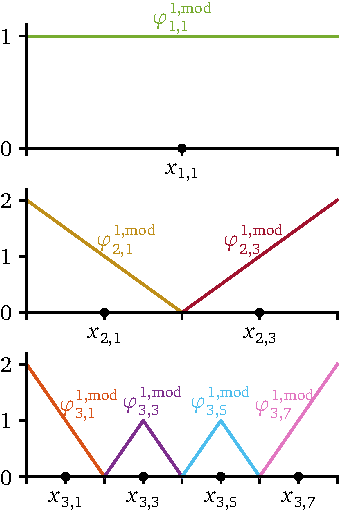
\includegraphics{hierarchicalBasis_3}%
  \caption[%
    Modified hierarchical hat functions%
  ]{%
    Modified hierarchical hat functions $\bspl[\modified]{l',i'}{1}$
    ($l' \le l$, $i' \in \hiset{l'}$) up to level $l = 3$.%
  }%
  \label{fig:modifiedHat}%
\end{SCfigure}
